%
\hsection{Relationship Diagrams}%
\FloatBarrier%
%
\begin{figure}%
\centering%
%
\subfloat[][%
To get to the \pgls{ERD} view, we click on \menu{Tools} and then \menu{Relationships}.%
\label{fig:factoryLibreOfficeBaseErd1Open}%
]{\tightbox{\includegraphics[width=0.49\linewidth]{\currentDir/factoryLibreOfficeBaseErd1Open}}}%
%
\floatSep%
%
\subfloat[][%
An \pgls{ERD} view of the tables in our \db\ appears. %
It is a bit cluttered, so we drag the tables around and resize them a bit.%
\label{fig:factoryLibreOfficeBaseErd2overview}%
]{\tightbox{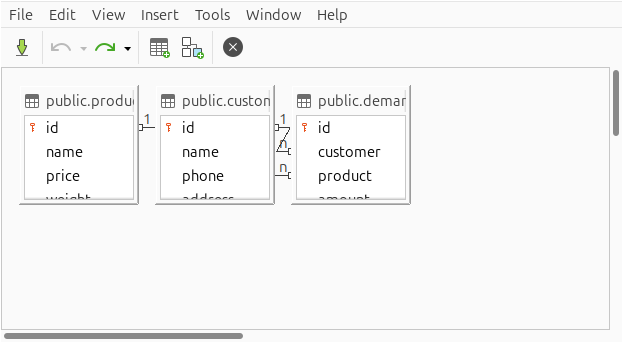
\includegraphics[width=0.49\linewidth]{\currentDir/factoryLibreOfficeBaseErd2overview}}}%
%
\floatRowSep%
%
\subfloat[][%
The \pgls{ERD} now looks very clean and illustrates the relationships between the tables in our \db.%
\label{fig:factoryLibreOfficeBaseErd3overviewRearranged}%
]{\tightbox{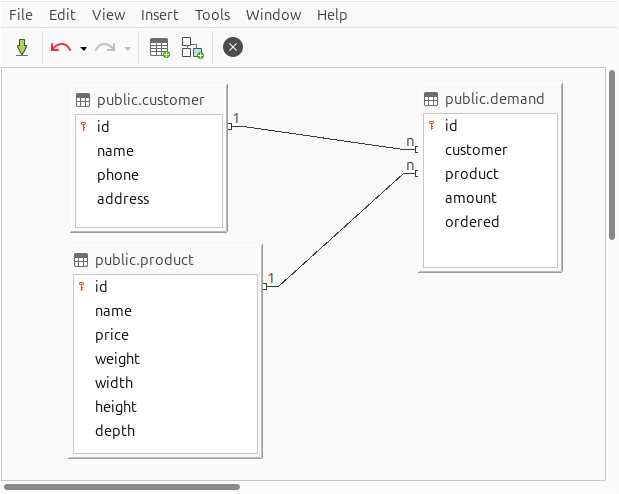
\includegraphics[width=0.7\linewidth]{\currentDir/factoryLibreOfficeBaseErd3overviewRearranged}}}%
%
%
\caption{Viewing an \pgls{ERD} of the tables and their relations in our \db\ in \libreofficeBase.}%
\label{fig:factoryLibreOfficeBaseERD}%
%
\end{figure}%
%
An important tool in \db\ design are \pglspl{ERD}.
\pglspl{ERD} are normally used when we design a \db.
They are visual representations of the objects and the relationships between them.
In the domain of \dbs, the objects could be tables and the relationships could be foreign key relationships.
It makes a lot of sense to first create a model of the real-world objects or information that we want to store in the \db.
Once we have modeled a \inQuotes{customer} and a \inQuotes{product}, we can model the information what consitutes a \inQuotes{demand} and how it is related to the previous two concepts.
This model, maybe drawn as \pgls{ERD}, can then be translated to a \db\ schema.
We can then construct the \db\ based on this design.

In this example, we did not do that.
We wanted to see action as quickly as possible and disregarded any concern about efficient design.
This example is not about fancy stuff, it is about exploring the world of \dbs.

Let's say that we did indeed design a \db\ based on entities modeled in a \pgls{ERD}.
The \db\ is created via \sql\ commands.
The tables correctly represent the model painted as \pgls{ERD}.
Then, the information in the \pgls{ERD} is also present in the \db.
It is reflected the structure of the tables and the foreign keys.
If this is true, then we should be able to reconstruct the \pgls{ERD} at least partially from a \db.
Of course, we cannot reconstruct the semantics, i.e., the meaning behind the relationships and objects.
But we can well reconstruct the objects and relationships on a purly syntactical level.

\libreofficeBase\ can do that.
Assume that we still have our \libreofficeBase\ \pgls{GUI} open, connected to our factory~\db.
We open the menu~\menu{Tools} and then click on \menu{Relationships}, as illustrated in \cref{fig:factoryLibreOfficeBaseErd1Open}.
This opens a very cluttered diagram view.
This view includes all three tables that we designed in our \db, but in~\cref{fig:factoryLibreOfficeBaseErd2overview} they are not neatly arranged.

We can click on them, though, and drag them around.
We can also drag the bottom edges of the tables and expand them.
After some re-arranging, we get indeed a very nice overview on our \db\ in \cref{fig:factoryLibreOfficeBaseErd2overview}.

We can see that the \sqlil{id} columns are the primary keys of the tables.
Furthermore, we see that each \sqlil{id} value in table \sqlil{customer} can be related to $n$~\sqlil{customer} values in table~\sqlil{demand}.
The same holds for each \sqlil{id} value in table \sqlil{product}, which can be related to $n$~\sqlil{product} values in table~\sqlil{demand}.
This \pgls{ERD} is a really overview on the structure of our \db.
And it is automatically generated for us by the \libreofficeBase\ \pgls{GUI}.
If our \db\ was more complex, with more tables and relationships, this illustration could be quite helpful.
Imagine that we designed the \db\ and a few years later we would move to another department and hand over the administration of this \db\ to a new \pgls{dba}.
They could then very quickly get an idea about the structure and relationships in the \db, without the need to dig through our \sql\ scripts.%
%
\FloatBarrier%
\endhsection%
%
